\documentclass{beamer}

\usepackage[utf8]{inputenc}
%\usepackage{adjustbox}
\usepackage[export]{adjustbox}
\usepackage{booktabs}
%\usepackage{ctex}
\usepackage{graphicx}
\usepackage{subcaption}

\captionsetup{compatibility=false}

\graphicspath{ {images/} }

\usetheme{Madrid}

\title[OJ user behavior]{The User Behavior On Online Judge Website }
\author[yiyuezhuo]{yueyi zhuo}
\institute[SICNU]{School of Mathematical,Sichuan Normal University}
\date{2017}

\begin{document}

\frame{\titlepage}

\begin{frame}

\frametitle{What is online judge(oj)?}

An online judge is an online system to test programs in programming contests. They are also used to practice for such contests. Many of these systems organize their own contests.

The system can compile and execute code, and test them with pre-constructed data. Submitted code may be run with restrictions, including time limit, memory limit, security restriction and so on. The output of the code will be captured by the system, and compared with the standard output. The system will then return the result. When mistakes were found in a standard output, rejudgement using the same method must be made.

Online Judges have ranklists showing users with the biggest number of accepted solutions and shortest execution time for a particular problem. \footnote{Wikipedia https://en.wikipedia.org/wiki/Online\_judge}

\end{frame}

\begin{frame}
\frametitle{Euler project}
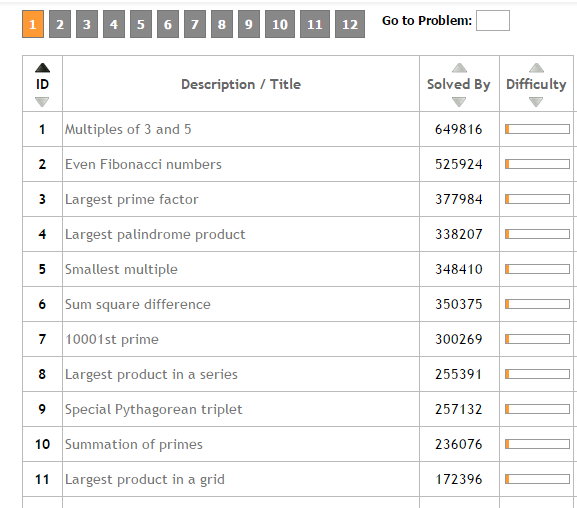
\includegraphics[scale=0.55]{euler-oj.png}
\end{frame}

\begin{frame}
\frametitle{leetcode OJ}
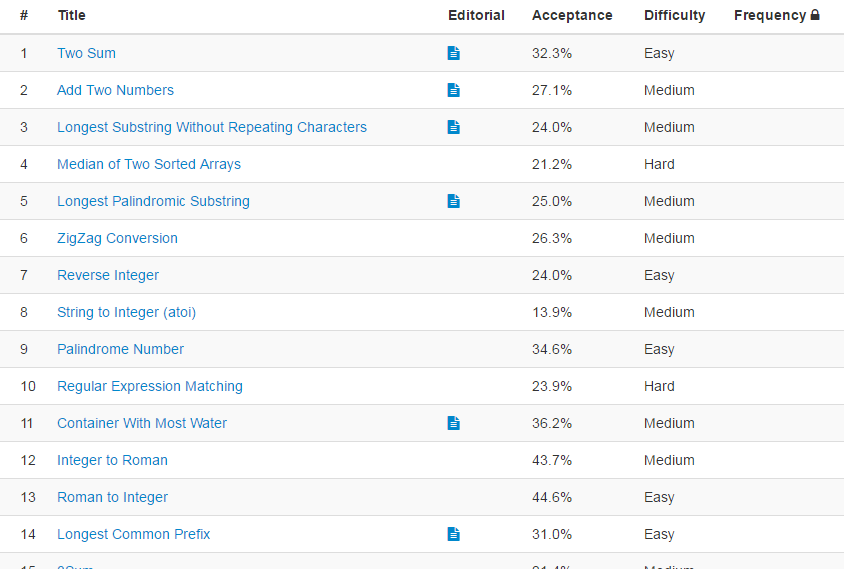
\includegraphics[scale=0.4]{leetcode-oj.png}
\end{frame}


\begin{frame}
\frametitle{Sicnu OJ}
\includegraphics[scale=0.5]{SICNU-oj.png}
\end{frame}

\begin{frame}
\frametitle{Some problem in Real world}

The data listed on the list looks very interesting. These're a number of insights for user behavior which 
can generalize to online education service. For example:

Why number of solved sequence looks like this? If we provide online education product as same as those oj, 
and observe such series, does it mean our product fail or extra-success?

\begin{figure}[h]
 
\begin{subfigure}{0.45\textwidth}
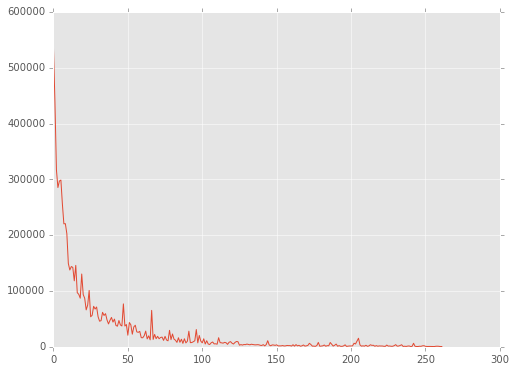
\includegraphics[width=0.9\linewidth, height=4cm]{solved-seq1.png} 
\caption{Solved number series}
\label{fig:subim1}
\end{subfigure}
\begin{subfigure}{0.45\textwidth}
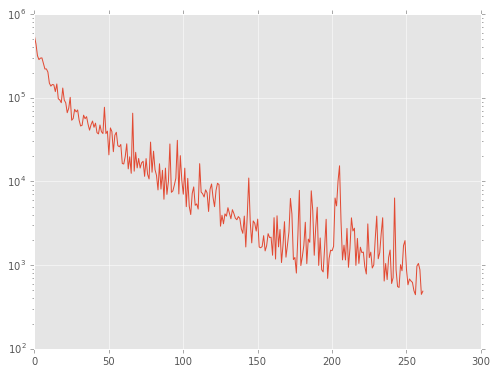
\includegraphics[width=0.9\linewidth, height=4cm]{solved-seq2.png}
\caption{Log solved number series}
\label{fig:subim2}
\end{subfigure}
 
\caption{Caption for this figure with two images}
\label{fig:image2}
\end{figure}

\end{frame}

\begin{frame}

\frametitle{Identify}

Is it signicant to put difficulty problem on the behind those easy problem 
if we want keep our user happy and not be shocked by those monster? It make sense
for online education to maintain user interest in their study process. For technically speaking:
According to data, do we observe the fact that a hard problem cause a temporary 
or continued solved number decrease,
although we have controlled other effect? 
How do we control other effect to identify the shock from hard problem?

There's a baseline regression have been run to 

\end{frame}

\begin{frame}

\frametitle{Model 1}

$$
solve_i = \beta_0 + \beta_1 id_i + \beta_2 diff_i + \epsilon_i
$$

where $id_i$ is the id of problem $i$, $diff_i$ is difficulty measure given by Project Euler.

\begin{center}
\scalebox{0.5}[0.5]{
\begin{tabular}{lclc}
\toprule
\textbf{Dep. Variable:}    &      solve       & \textbf{  R-squared:         } &    0.331  \\
\textbf{Model:}            &       OLS        & \textbf{  Adj. R-squared:    } &    0.325  \\
\textbf{Method:}           &  Least Squares   & \textbf{  F-statistic:       } &    63.95  \\
\textbf{Date:}             & Mon, 10 Apr 2017 & \textbf{  Prob (F-statistic):} & 2.68e-23  \\
\textbf{Time:}             &     22:53:04     & \textbf{  Log-Likelihood:    } &  -3224.6  \\
\textbf{No. Observations:} &         262      & \textbf{  AIC:               } &    6455.  \\
\textbf{Df Residuals:}     &         259      & \textbf{  BIC:               } &    6466.  \\
\textbf{Df Model:}         &           2      & \textbf{                     } &           \\
\textbf{Covariance Type:}  &    nonrobust     & \textbf{                     } &           \\
\bottomrule
\end{tabular}
%\caption{OLS Regression Results}
}
\scalebox{0.5}[0.5]{
\begin{tabular}{lccccc}
\toprule
                   & \textbf{coef} & \textbf{std err} & \textbf{t} & \textbf{P$>$$|$t$|$} & \textbf{[95.0\% Conf. Int.]}  \\
\midrule
\textbf{Intercept} &    9.401e+04  &     6678.292     &    14.077  &         0.000        &      8.09e+04  1.07e+05       \\
\textbf{id}        &    -479.7585  &       90.521     &    -5.300  &         0.000        &      -658.008  -301.509       \\
\textbf{diff}      &     -60.2227  &      266.704     &    -0.226  &         0.822        &      -585.406   464.961       \\
\bottomrule
\end{tabular}
}
\scalebox{0.5}[0.5]{
\begin{tabular}{lclc}
\toprule
\textbf{Omnibus:}       & 270.575 & \textbf{  Durbin-Watson:     } &    0.077  \\
\textbf{Prob(Omnibus):} &   0.000 & \textbf{  Jarque-Bera (JB):  } & 8178.806  \\
\textbf{Skew:}          &   4.299 & \textbf{  Prob(JB):          } &     0.00  \\
\textbf{Kurtosis:}      &  28.986 & \textbf{  Cond. No.          } &     317.  \\
\bottomrule
\end{tabular}
}
\end{center}

\end{frame}

\begin{frame}

We can see the estimated effect of diff is negative but not be signicant. The result does not adapt by theory,
and DW statistic is too low which imply possibility that autocorrelation exist in model. 
Let we try to apply log transform on $solve$ to reduce the effect and to make estimated value more precise.

\begin{figure}[h]
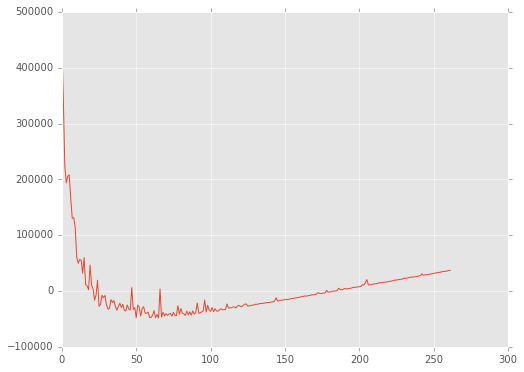
\includegraphics[width=0.5\textwidth, inner]{model1-resid.png}
\caption{Plot of residuals of model 1}
\end{figure}

\end{frame}

\begin{frame}

\frametitle{Model 2}

$$
\log(solve_i) = \beta_0 + \beta_1 id_i + \beta_2 diff_i + \epsilon_i
$$

\begin{center}
\scalebox{0.5}[0.5]{
\begin{tabular}{lclc}
\toprule
\textbf{Dep. Variable:}    &    log(solve)    & \textbf{  R-squared:         } &     0.943  \\
\textbf{Model:}            &       OLS        & \textbf{  Adj. R-squared:    } &     0.943  \\
\textbf{Method:}           &  Least Squares   & \textbf{  F-statistic:       } &     2150.  \\
\textbf{Date:}             & Mon, 10 Apr 2017 & \textbf{  Prob (F-statistic):} & 4.94e-162  \\
\textbf{Time:}             &     23:27:00     & \textbf{  Log-Likelihood:    } &   -128.21  \\
\textbf{No. Observations:} &         262      & \textbf{  AIC:               } &     262.4  \\
\textbf{Df Residuals:}     &         259      & \textbf{  BIC:               } &     273.1  \\
\textbf{Df Model:}         &           2      & \textbf{                     } &            \\
\textbf{Covariance Type:}  &    nonrobust     & \textbf{                     } &            \\
\bottomrule
\end{tabular}
%\caption{OLS Regression Results}
}
\scalebox{0.5}[0.5]{
\begin{tabular}{lccccc}
\toprule
                   & \textbf{coef} & \textbf{std err} & \textbf{t} & \textbf{P$>$$|$t$|$} & \textbf{[95.0\% Conf. Int.]}  \\
\midrule
\textbf{Intercept} &      11.4369  &        0.049     &   232.406  &         0.000        &        11.340    11.534       \\
\textbf{id}        &      -0.0081  &        0.001     &   -12.179  &         0.000        &        -0.009    -0.007       \\
\textbf{diff}      &      -0.0407  &        0.002     &   -20.685  &         0.000        &        -0.045    -0.037       \\
\bottomrule
\end{tabular}
}
\scalebox{0.5}[0.5]{
\begin{tabular}{lclc}
\toprule
\textbf{Omnibus:}       & 117.312 & \textbf{  Durbin-Watson:     } &     0.197  \\
\textbf{Prob(Omnibus):} &   0.000 & \textbf{  Jarque-Bera (JB):  } &   466.808  \\
\textbf{Skew:}          &   1.888 & \textbf{  Prob(JB):          } & 4.30e-102  \\
\textbf{Kurtosis:}      &   8.339 & \textbf{  Cond. No.          } &      317.  \\
\bottomrule
\end{tabular}
}
\end{center}

\end{frame}

\begin{frame}

New model make $diff$ significant but DW statistic still be too small (0.197 from 0.07). 
Since $diff$ is not a real quantity index which take value as 5, 10, etc for no reason,
we replace it to two new dummy variables $diff\_mid$ and $diff\_hard$. 
$diff\_mid_i=1$ if $diff > 25$,else $diff\_mid_i=0$.
$diff\_hard_i=1$ if $diff > 50$,else $diff\_hard_i=0$.


\begin{figure}[h]
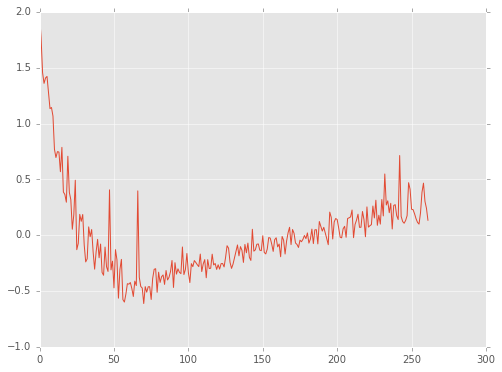
\includegraphics[width=0.5\textwidth, inner]{model2-resid.png}
\caption{Plot of residuals of model 2}
\end{figure}


\end{frame}

\end{document}